\documentclass[a4paper]{article}

\usepackage{times} \usepackage{tikz} \usepackage[margin=0cm]{geometry}
\usepackage{graphicx} \usepackage{anyfontsize} \usepackage{fancyhdr}
\usepackage{indentfirst} \usepackage{amsmath} \usepackage[spanish]{babel}
\usepackage[utf8]{inputenc} \usepackage[explicit]{titlesec} \usepackage{etoolbox} 
\usepackage{multicol}

\author{} \date{} \title{}

\newcommand{\longsection}[2]{\section[#1]{\parbox{\columnwidth}{#1}}}

\newcommand{\saltoPag}{\newpage \noindent \thispagestyle{fancy}}

\begin{document}
\thispagestyle{empty}
\begin{tikzpicture}[remember picture, overlay]
    \pgftransformshift{\pgfpoint{0cm}{0cm}}
    \draw [line width=2pt](1cm,-1cm) -- (1cm,-27.7cm) -- (14cm, -27.7cm) -- (14cm, -1cm) -- (1cm, -1cm);
    \draw[line width=2pt] (15cm, -27.7cm) -- (19cm,-27.7cm) -- (19cm, -1cm) -- (15cm, -1cm) --  (15cm, -27.7cm);
    \node [line width=2pt] at (17cm, -3.5cm) {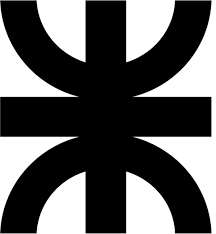
\includegraphics[width=3cm]{../imagenes/utn.png}};
	\node [line width=2pt] at (7.5cm, -7.5cm) {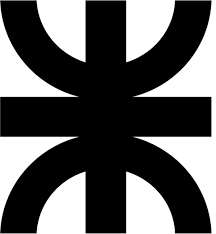
\includegraphics[width=6cm]{../imagenes/utn.png}};
    \node at (17cm, -7cm) {\scalebox{5}{\textbf{U}}};
    \node at (17cm, -9cm) {\scalebox{5}{\textbf{T}}};
    \node at (17cm, -11cm) {\scalebox{5}{\textbf{N}}};
    \node at (17cm, -14cm) {\scalebox{5}{\textbf{F}}};
    \node at (17cm, -16cm) {\scalebox{5}{\textbf{R}}};
    \node at (17cm, -18cm) {\scalebox{5}{\textbf{C}}};
    \node at (7.25cm, -12cm) {\scalebox{2.5}{\textbf{Resumen $1^{er} parcial$}}};
    \node at (7.5cm, -24cm) {
	\begin{minipage}[c]{12cm}
	    \begin{itemize}
            \raggedright
            \vspace{1.5cm}
            \item \fontsize{12}{12}\selectfont \textbf{Autor:} Marcos Raúl Gatica \\
            \item \fontsize{12}{12}\selectfont \textbf{Curso:} 2R1 \\
            \item \fontsize{12}{12}\selectfont \textbf{Asignatura:} Física electrónica.  \\
            \item \fontsize{12}{12}\selectfont \textbf{Institución:} Universidad Tecnológica Nacional - Facultad Regional de Córdoba. \\
        \end{itemize}
    \end{minipage}};

\end{tikzpicture}

\renewcommand{\theenumi}{\roman{enumi}}
\renewcommand{\normalsize}{\fontsize{12}{18}\selectfont}
\newgeometry{margin=2cm}
\fancyhf{}
\renewcommand{\headrulewidth}{0pt}
\renewcommand{\footrulewidth}{0.4pt}
\fancyfoot[R]{[Gatica M.] [\textbf{pág.\ \thepage}]}
\setlength{\footskip}{1.5cm}

\newpage
\thispagestyle{empty}
\text{}

\titleformat{\section}[hang]{\fontsize{12}{12}\bfseries}{\thesection.}{0.5em}{\underline{#1}}

\newpage
\newpage
\thispagestyle{empty}
\setcounter{page}{0}
\tableofcontents
\saltoPag
\setlength{\columnseprule}{0.4pt}
\setlength{\columnsep}{0.5cm}

\begin{multicols}{2}
    \section{UNIDAD 1}
        \subsection{Leyes básicas: electricidad y magnetismo}
            \textbf{\underline{Conceptos - electricidad}} \\
                \begin{itemize}
                    \item \underline{Electrostática}: interacción entre dos cargas en reposo. \\
                    \item \underline{Tipos de cargas}: positivas y negativas, que mutuamente se atraen. La existencia de las mismas se dedujeron por experimentos. \\
                    \item \underline{Atracción y repulsión de cargas}: solo se tiene en cuenta el signo algebraico de las cargas. P-N se atraen y P-P o N-N se repelen. \\
                    \item \underline{Principio de consevación de la energía}: La suma algebraica de todas las cargas eléctricas en cualquier sistema cerrado es constante. \\
                        \indent En cualquier proceso de carga, esta no se crea ni se destruye, solo se transfiere de un cuerpo a otro. \\
                    \item \underline{Conductores}: materiales que permiten el movimiento libre y ordenado de los electrones sobre los átomos de un conductor eléctrico de diferente energía de potencial. \\
                    \item \underline{Aislantes}: no permiten el flujo de electrones. \\
                        \indent Nótese la comparación de un sólido metálico (donde el flujo es posible en ''la nube de electrones''), y un sólido iónico. \\
                    \item \underline{Carga por inducción}: Dada una esfera eléctricamente neutra al principio, si le acercamos una barra con carga positiva, los electrones se acercan a ella y en la esfera se inducen dos cargas: un lado queda eléctricamente negativo mientras que el otro tiene un déficit de cargas negativas, se ''posietiviza''.
                \end{itemize}
                \begin{center} 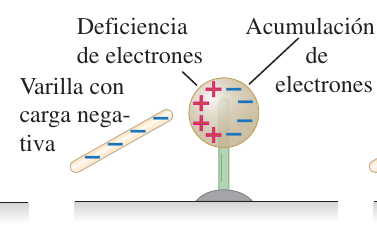
\includegraphics[width=3.5cm]{../imagenes/esferaInduccion.png} \end{center}

            \textbf{\underline{Ley de Coulomb}} \\[10pt]
                \indent La magnitud de la fuerza eléctrica entre dos cargas puntuales es directamente proporcional al producto de las cargas e inversamente proporcional al cuadrado de la distancia que las separa.

                \begin{center} $\vec{F} = k{\frac{q_1q_2}{r^2}}$ \end{center}

                \textbf{\underline{Ley de Gauss para el campo eléctrico}} \\[10pt] \indent Dada cualquier distribución general de carga, rodeamos la misma con una superficie imaginaria y analizamos los efectos del campo eléctrico en los puntos de la superficie. \\ 

                \underline{Carga y flujo eléctrico}: Se introduce el concepto de ''superficie cerrada'', aquella que engloba un campo eléctrico. Para Determinar el campo aquí, se coloca una carga puntual y se evalúa la fuerza en relación al campo: \\
                    \begin{center} $\vec{E} = \frac{\vec{F}}{q}$ \end{center}

                \underline{Flujo eléctrico y carga encerrada}: Dada una superficie cerrada con un campo eléctrico, podemos determinar un ''flujo'', digamos cómo salen esos vectores de la superficie. \\ \indent El flujo será positivo si las líneas de campo ''entran'' a la superficie, en caso contrario serán negativos.
                    \begin{center} 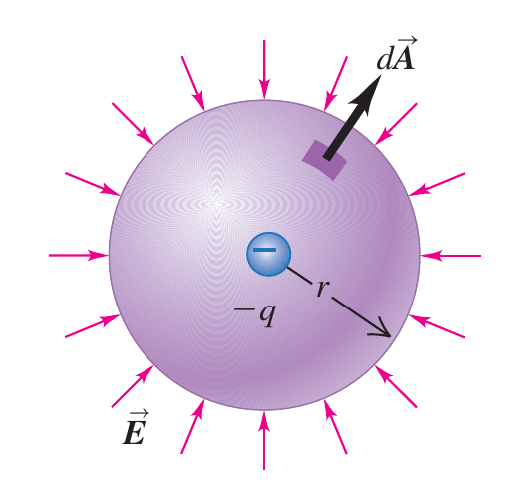
\includegraphics[width=3.5cm]{../imagenes/campoElectricoEntrante.png} \end{center}
                    \begin{center} 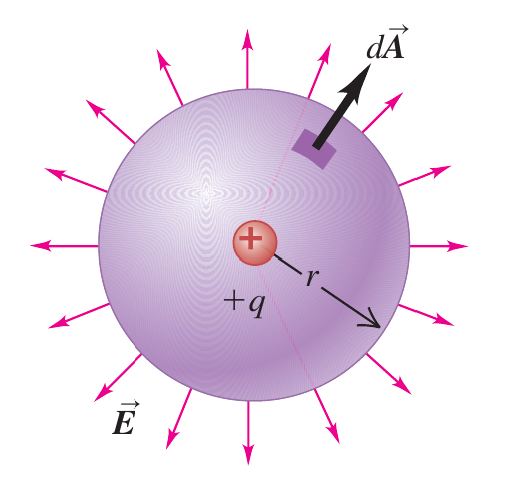
\includegraphics[width=3.5cm]{../imagenes/campoElectricoSaliente.png} \end{center}
                    
                    \begin{itemize}
                        \item La carga neta dentro de la superficie será 0 cuando existan la misma cantidad de cargas positivas como negativas, o no haya cargas.
                        \item Una carga es positiva o negativa según la dirección del flujo y con respecto a cargas de prueba.
                        \item Las cargas ''fuera'' de la superficie no provocan flujo en la misma.
                        \item El flujo eléctrico es proporcional a la cantidad de carga neta contenida dentro de la superficie y no por el tamaño de la misma.
                    \end{itemize}
                \underline{Cálculo del flujo eléctrico} 
                    \begin{itemize}
                        \item \underline{Campo uniforme}: \begin{center} $\phi = \vec{E} \vec{N} \cos(\theta)$ \\[10pt] 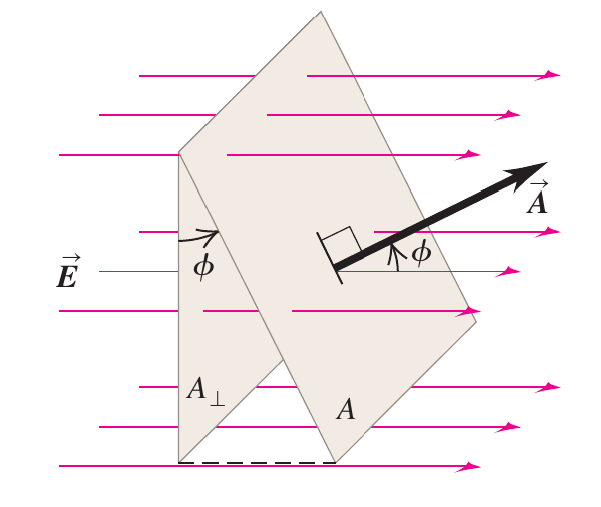
\includegraphics[width=3.5cm]{../imagenes/flujoCampoElectricoUniforme.png} \end{center} 
                        \saltoPag
                        \item \underline{Campo no uniforme}: \begin{center} $\phi = \int \vec{E}\cos(\theta)d\vec{A}$ \\[10pt]\end{center} \indent Aplicable a superficies irregulares o no lineales, como a campos eléctricos que varían de un punto de la superficie a otro.
                    \end{itemize}
                \underline{Formulación gral: Ley de Gauss para el campo eléctrico}: 
                    \begin{center} $\phi_{electrico} = \oint \vec{E_\perp}d\vec{A} = \frac{\sum Q_{int}}{\epsilon_0}$ \end{center}
                    \begin{itemize}
                        \item Las líneas de campo eléctrico comienzan y terminan dentro de una región del espacio sólo cuando en esa región existe carga.
                        \item Cargas negativas provocan sumideros donde las líneas de campo entran a la superficie.
                        \item Cargas positivas provocan fuentes donde las líneas de campo salen de la superficie.
                    \end{itemize}
            \textbf{\underline{Conceptos - Magnetismo}}
                \begin{itemize}
                    \item Una carga o corriente crea un campo magnético en el espacio circulante, además de un campo eléctrico.
                    \item El campo magnético ejerce una fuerza $\vec{F}$ sobre cualquier otra carga o corriente en el mismo.
                \end{itemize}
                \underline{Fuerzas magnéticas en cargas móviles} \\[10pt]
                    \begin{itemize}
                        \item La magnitud de la fuerza es proporcional a la magnitud de la carga.
                        \item La magnitud de la fuerza es proporcional a la intensidad del campo $\vec{B}$
                        \item La fuerza magnética depende de la velocidad de la partícula.
                        \item La fuerza $\vec{F}$ es perpendicular al campo y a la velocidad.
                    \end{itemize}
                    \begin{center} 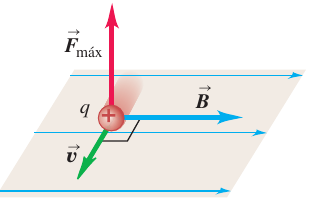
\includegraphics[width=3.5cm]{../imagenes/ejesCampoMagnetico.png} \\ \end{center} 
                    
                \underline{Fuerzas magnéticas y eléctricas} 
                    \begin{center} $\vec{F} = q(\vec{V}\vec{E} \times \vec{B})$ \end{center}
                \underline{Ley de Gauss para el magnetismo} \\[10pt]
                    \indent El flujo magnético $\phi_B$ se determina de la misma forma que el flujo eléctrico. \\
                    \begin{center} 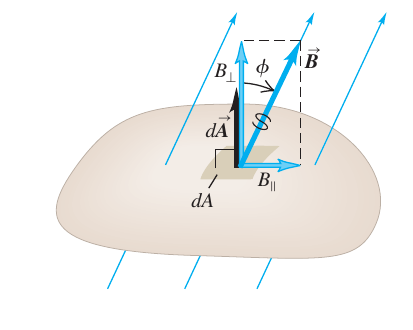
\includegraphics[width=4cm]{../imagenes/flujoCampoMagnetico.png} \end{center}
                    \indent Desarrollo:
                    \begin{center}
                        $d\phi_B = \vec{B}\cos(\theta)d\vec{A}$ \\[10pt]
                        $\phi_B = \int \vec{B}\cos(\theta)d\vec{A}$ \\[10pt]
                    \end{center}
                    \indent Para un campo magnético uniforme podemos decir:
                    \begin{center} $\phi_B = B\cos(\theta)\Delta \vec{A}$ \end{center}
                    \indent Dado a que no existen los monopolos magnéticos, y que todas las líneas del campo magnético entran y salen, se puede decir:
                    \begin{center} $\oint \vec{B} d\vec{A} = 0$ \end{center}
                \underline{Ley de Faraday} \\[10pt]
                    \indent La FEM inducida en una espira cerrada es igual al negativo de la tasa de cambio del flujo magnético a través de una espira con respecto al tiempo.
                    \begin{center} $\epsilon = - \frac{d\phi_B}{dt}$ \end{center}
                    \indent Determinar el signo de las variables:
                    \begin{itemize}
                        \item Definir una dirección positiva para el vector área $\vec{A}$
                        \item A partir de las direcciones de $\vec{A}$ y del vector de campo magnético $\vec{B}$, determinar el signo del flujo y la tasa de cambio del mismo.
                        \item El signo de la FEM viene dado por si el flujo es creciente tal que su tasa de cambio es positiva, la FEM es negativa.
                    \end{itemize}
                    \begin{center} 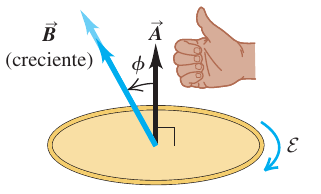
\includegraphics[width=4cm]{../imagenes/direccionFEMInducida.png} \end{center}
                \underline{Ley de Lenz} \\[10pt]
                    \begin{itemize}
                        \item Es un método alternativo para determinar la dirección de la FEM inducida, su principio se puede obtener por la Ley de Faraday.
                        \item ''El campo magnético, concretamente su dirección, genera una FEM inducida, y el sentido de esta última de opone a la causa que lo generó.''
                        \item Es una consecuencia del principio de conservación de la energía.
                    \end{itemize}
                    \saltoPag
                \underline{Fuerzas de Lorenz} \\[10pt]
                    \begin{itemize}
                        \item $\vec{F} = q \vec{E}$ \hspace{5mm} [Campo eléctrico] \\[5pt]
                        \item $\vec{F} = q\vec{V} \times \vec{B}$ \hspace{5mm}[Campo magnético] \\[5pt]
                    \end{itemize}
                \underline{Ley de Ampere} \\[10pt]
                    \begin{itemize}
                        \item \textbf{Corriente de conducción}: velocidad de flujo de electrones sobre la sección de un conductor.
                            \begin{center} $I_C = \int_{A cond.} Jd\vec{A}$ \end{center}
                        \item \textbf{Ley de Ampere incompleta}: ''Los campos magnéticos son generados por las corrientes de conducción en materiales conductores''
                            \begin{center} $\nabla \times \vec{B} = \mu_0 J$ \end{center}
                        \item \textbf{Corrientes de desplazamiento}: aparece en lugares donde un campo eléctrico varía, pero no hay cargas presentes.
                            \begin{center} $I_0 = \epsilon_0 \frac {d\phi_{\vec{E}}}{dt}$ \end{center}
                        \item \textbf{Ley de Ampere-Maxwell}: 
                            \begin{center} $\nabla \times \vec{B} = (I_C + I_D) = \mu_0 (J + \epsilon_0 \frac{d\phi_{\vec{E}}}{dt})$ \end{center}
                    \end{itemize}
        \subsection{Ecuaciones de Maxwell}
            \indent Son un conjunto de cuatro ecuaciones que describen el comportamiento de los campos eléctrico y magnético ante cargas y corrientes. 
            \begin{enumerate}
                \item Gauss para los campos eléctricos:
                    \begin{center} $\oint \vec{E} d\vec{A} = \frac{Q_{int}}{\epsilon_0}$ \end{center}
                \item Gauss para los campos magnéticos:
                    \begin{center} $\oint \vec{B} d\vec{A} = 0 $ \end{center}
                \item Faraday:
                    \begin{center} $\oint \vec{E} d\vec{l} = - \frac{d\phi_{\vec{B}}}{dt}$ \end{center}
                \item Ampere-Maxwell:
                    \begin{center} $\oint \vec{B} d\vec{l} = I_C + I_D$ \end{center}
            \end{enumerate}
            \subsection{Demostraciones}
                \underline{\textbf{Relación velocidad de la luz y las E.M.}}
                    \begin{itemize}
                        \item Objetivo: buscar la velocidad de propagación de la luz en el vació y en un entorno sin cargas (lo que implica $\vec{\rho} = 0$ y $\vec{J} = 0$)
                        \item Desarrollo:
                            \begin{enumerate}
                                \item Tomando las leyes de Faraday y Ampere-Maxwell, podemos buscar la ecuación de onda para ambos campos:
                                \begin{center}
                                    $\nabla \times \vec{E} = - \frac{\partial \vec{B}}{\partial t}$ \hspace{5mm} [Faraday] \\[5pt]
                                    $\nabla (\nabla \times \vec{E}) = \nabla (- \frac{\partial \vec{B}}{dt})$ \hspace{5mm} [Rotacional a ambos lados] \\[5pt]                             
                                \end{center}
                                \item Tomamos el primer miembro de la ecuación anterior y vemos que:
                                    \begin{center} $\nabla (\nabla \times \vec{E}) = \nabla (\nabla \vec{E}) - {\nabla}^2 \vec{E}$ [Teorema divergencia] \\[5pt ]\end{center}
                                    Por ley de Gauss para el campo eléctrico en un entorno sin cargas: $\nabla \vec{E} = 0$ \\[5pt]
                                    \begin{center} $\nabla (\nabla \times \vec{E}) = - {\nabla}^2 \vec{E}$ \end{center}
                                \item Ahora se toma el segundo miembro de la ecuación del principio (ítem I):
                                    \begin{center} 
                                        $-\nabla \times \frac{\partial \vec{B}}{\partial t} = -\frac{\partial}{\partial t} (\nabla \times \vec{B})$ \hspace{5mm} [Amp-Max] \\[5pt]
                                        $-\nabla \times \frac{\partial \vec{B}}{\partial t} = -\frac{\partial}{\partial t} (\mu_0 \epsilon_0 \frac{\partial \vec{E}}{\partial t}) $ \\[5pt]
                                        $-\nabla \times \frac{\partial \vec{B}}{\partial t} = - \mu_0 \epsilon_0 \frac{\partial ^2 \vec{E}}{\partial t^2}$
                                    \end{center}
                                \item Igualamos las dos ecuaciones que logramos obtener para llegar a:
                                    \begin{center}
                                        $-\nabla ^2\vec{E} = -\mu_0 \epsilon_0 \frac{\partial ^2 \vec{E}}{\partial t^2}$ \\[5pt]
                                        $\nabla ^2\vec{E} = \mu_0 \epsilon_0 \frac{\partial ^2 \vec{E}}{\partial t^2}$ \\[5pt]
                                    \end{center}

                                \item Comparado a la original ($\nabla ^2\vec{E} = v^{-2} \frac{\partial ^2 \vec{E}}{\partial t ^2}$), vemos que esto describe una onda electromagnética en el vacío y podemos hacer la asociación:
                                    \begin{center} $v^{-2} = \mu_0 \epsilon_0$ \\[5pt] $v = \frac{1}{\sqrt{\mu_0 \epsilon_0}}$ \hspace{5mm} [Vel. de la luz en el vacío] \end{center}
                            \end{enumerate}
                    \end{itemize}
                    \underline{\textbf{Ec. Maxwell (integral $\rightarrow$ diferencial)}}
                    \begin{itemize}
                        \item Ley de Gauss para el campo eléctrico:
                            \begin{enumerate}
                                \item Forma integral:
                                    \begin{center} $\oint_S \vec{E} d\vec{A} = \frac{Q_{int}}{\epsilon_0}$ \end{center}
                                \item Aplicar teorema de la divergencia en el primer miembro, siendo:
                                    \begin{center} $\oint_S \vec{E} d\vec{A} = \iiint_V (\nabla \vec{E})dV$ \end{center}
                                \item Combinando esto con la densidad de carga $\rho = \frac{Q_{int}}{V}$, se obtiene:
                                    \begin{center} $\nabla \vec{E} = \frac{\rho}{\epsilon_0}$ \end{center}
                            \end{enumerate}
                        \item Ley de Gauss para el campo magnético:
                            \begin{enumerate}
                                \item Forma integral:
                                    \begin{center} $\oint_S \vec{B} d\vec{A} = 0$ \end{center}
                                \item Aplicando el teorema de divergencia en el primer miembro:
                                    \begin{center} $\oint_S \vec{B} d\vec{A} = \iiint (\nabla \vec{B})dV$ \end{center}
                                \item Se sabe entonces que:
                                    \begin{center} $\nabla \vec{B} = 0$ \end{center}
                            \end{enumerate}
                        \item Faraday:
                            \begin{enumerate}
                                \item Forma integral:
                                    \begin{center} $\oint_C \vec{E} d\vec{l} = - \frac{d\phi_{\vec{B}}}{dt}$ \end{center}
                                \item Aplicando el teorema de Stokes en el primer miembro:
                                    \begin{center} $\oint_C \vec{E} d\vec{l} = \iint (\nabla \times \vec{E}) \vec{A}$ \end{center}
                                \item Dado que $- \frac{d\phi_{\vec{B}}}{dt}$ es la tasa de cambio de flujo magnético, se obtiene:
                                    \begin{center} $\nabla \times \vec{E} = -\frac{\partial \vec{B}}{\partial t}$ \end{center}
                            \end{enumerate}
                        \item Ley Ampere-Maxwell:
                            \begin{enumerate}
                                \
                            \end{enumerate}
                    \end{itemize}
\end{multicols}

\end{document}


